%%%%%%%%%%%%%%%%%%%%%%%%%%%%%%%%%%%%%%%%%
% NIH Grant Proposal for the Specific Aims and Research Plan Sections
% LaTeX Template
% Version 1.1 (26/12/19)
%
% This template originates from:
% http://www.LaTeXTemplates.com
%
% Original author:
% Erick Tatro (erickttr@gmail.com) with modifications by:
% Vel (vel@latextemplates.com)
%
% Adapted from:
% J. Hrabe (http://www.magalien.com/public/nih_grants_in_latex.html)
%
% License:
% CC BY-NC-SA 3.0 (http://creativecommons.org/licenses/by-nc-sa/3.0/)
%
%%%%%%%%%%%%%%%%%%%%%%%%%%%%%%%%%%%%%%%%%

%----------------------------------------------------------------------------------------
%	PACKAGES AND OTHER DOCUMENT CONFIGURATIONS
%----------------------------------------------------------------------------------------

% \documentclass[11pt, notitlepage]{article} % Default font size and suppress title page
\documentclass[a4paper, 11pt, notitlepage]{report}

\usepackage[utf8]{inputenc} % Required for inputting international characters
\usepackage[T1]{fontenc} % Output font encoding for international characters
% A note on fonts: As of 2019, NIH allows Arial, Georgia, Helvetica, and Palatino Linotype. Georgia and Arial are commercial fonts so you will need to use XeLaTeX and have them installed on your machine to use them. Palatino & Helvetica are available as free LaTeX packages so select the one you want and comment out the other.
\usepackage{palatino} % Palatino font
\linespread{1.05} % A little extra line spread is better for the Palatino font
%\usepackage{helvet} % Helvetica font
\renewcommand*\familydefault{\sfdefault} % Use the sans serif version of the font
\usepackage[subpreambles=true]{standalone}
\usepackage{import}
\usepackage{longtable}

\usepackage{amsfonts, amsmath, amsthm, amssymb} % For math fonts, symbols and environments
\usepackage{graphicx} % Required for including images
\usepackage{booktabs} % Nice rules in tables
\usepackage{wrapfig} % Required for text to wrap around figures and tables
\usepackage[labelfont=bf]{caption} % Make figure numbering in captions bold
\usepackage[top=0.5in,bottom=0.5in,left=0.5in,right=0.5in]{geometry} % Page margins
\pagestyle{empty} % Suppress headers and footers

\hyphenation{ionto-pho-re-tic iso-tro-pic fortran} % Specifies custom hyphenation points for words or words that shouldn't be hyphenated at all

\author{
        Woon Jun Wei \textit{2200624} \\
        Benjamin Loh Choon How \textit{2201590} \\
        Wang Rongqi Richie \textit{2201942} \\
        Poon Xiang Yuan \textit{2200559} \\
        Low Hong Sheng Jovian \textit{2203654}\\
    }

\title{
  INF2007 - Mobile Application Develpopment - Project Design 
}
%----------------------------------------------------------------------------------------

\begin{document}

\maketitle

%----------------------------------------------------------------------------------------
%	Proposal Section
%----------------------------------------------------------------------------------------

\import{Sections/}{Proposal}

%----------------------------------------------------------------------------------------
%	User Stories Section
%----------------------------------------------------------------------------------------

\import{Sections/}{User_Stories}

%----------------------------------------------------------------------------------------
%	UI Prototypes Section
%----------------------------------------------------------------------------------------

% \newpage
\import{Sections/}{UI_Prototypes}

%----------------------------------------------------------------------------------------
%	Backlogs Section
%----------------------------------------------------------------------------------------

\import{Sections/}{Backlogs}

%----------------------------------------------------------------------------------------
%	Architecture Section
%----------------------------------------------------------------------------------------

\import{Sections/}{Software_Architecture}

%----------------------------------------------------------------------------------------
%	Appendix Section
%----------------------------------------------------------------------------------------
\appendix
\import{Appendix/}{Appendix_A}


%----------------------------------------------------------------------------------------
%	BIBLIOGRAPHY
%----------------------------------------------------------------------------------------

\newpage

\bibliography{Mobile_Project_Design} % Use the NIHGrant.bib file for the reference list, replace with your own
\bibliographystyle{ieee} % Use the custom nihunsrt bibliography style included with the template

%----------------------------------------------------------------------------------------

\end{document}

%----------------------------------------------------------------------------------------
%	SPECIFIC AIMS
%----------------------------------------------------------------------------------------

%\section*{Specific Aims}
%
%This is an example citation \cite{Tatro2013}. Lorem ipsum dolor sit amet, consectetur adipiscing elit. Praesent porttitor arcu luctus, imperdiet urna iaculis, mattis eros. Pellentesque iaculis odio vel nisl ullamcorper, nec faucibus ipsum molestie. Sed dictum nisl non aliquet porttitor. Etiam vulputate arcu dignissim, finibus sem et, viverra nisl. Aenean luctus congue massa, ut laoreet metus ornare in. Nunc fermentum nisi imperdiet lectus tincidunt vestibulum at ac elit. Nulla mattis nisl eu malesuada suscipit.
%
%Aliquam arcu turpis, ultrices sed luctus ac, vehicula id metus. Morbi eu feugiat velit, et tempus augue. Proin ac mattis tortor. Donec tincidunt, ante rhoncus luctus semper, arcu lorem lobortis justo, nec convallis ante quam quis lectus. Aenean tincidunt sodales massa, et hendrerit tellus mattis ac. Sed non pretium nibh. Donec cursus maximus luctus. Vivamus lobortis eros et massa porta porttitor.
%
%Fusce varius orci ac magna dapibus porttitor. In tempor leo a neque bibendum sollicitudin. Nulla pretium fermentum nisi, eget sodales magna facilisis eu. Praesent aliquet nulla ut bibendum lacinia. Donec vel mauris vulputate, commodo ligula ut, egestas orci. Suspendisse commodo odio sed hendrerit lobortis. Donec finibus eros erat, vel ornare enim mattis et. Donec finibus dolor quis dolor tempus consequat. Mauris fringilla dui id libero egestas, ut mattis neque ornare. Ut condimentum urna pharetra ipsum consequat, eu interdum elit cursus. Vivamus scelerisque tortor et nunc ultricies, id tincidunt libero pharetra. Aliquam eu imperdiet leo. Morbi a massa volutpat velit condimentum convallis et facilisis dolor.
%
%\begin{description}
%	\item[Aim 1: Really cool stuff.]{}
%	\item{1.1. First sub-aim with more details}
%	\item{1.2. Second sub-aim with more details.}  
%\end{description}
%
%\begin{description}
%	\item[Aim 2: Really cool stuff.]{}
%	\item{2.1. First sub-aim with more details.}
%	\item{2.2. Second sub-aim with more details.}
%\end{description}
%
%\begin{description}
%	\item[Aim 3: Really cool stuff.]{ }
%	\item{3.1. First sub-aim with more details.}
%	\item {3.2. Second sub-aim with more details.}
%	\item{3.3. Third sub-aim with more details.}
%\end{description}
%
%In hac habitasse platea dictumst. Curabitur mattis elit sit amet justo luctus vestibulum. In hac habitasse platea dictumst. Pellentesque lobortis justo enim, a condimentum massa tempor eu. Ut quis nulla a quam pretium eleifend nec eu nisl. Nam cursus porttitor eros, sed luctus ligula convallis quis. Nam convallis, ligula in auctor euismod, ligula mauris fringilla tellus, et egestas mauris odio eget diam. Praesent sodales in ipsum eu dictum.

%----------------------------------------------------------------------------------------
%	SIGNIFICANCE
%----------------------------------------------------------------------------------------

%\newpage
%
%\section*{A. Significance}
%
%\begin{description} % For subheadings within a section, this template uses the {description} environment, it is not obtrusively large like a \subsection; and facilitates a brief optional subtitle; and it will wrap around figures and tables; it also has a decent amount of whitespace above/below which is less than for a section heading
%	\item[A.1. Instructions.]{Optional subtitle}
%\end{description}
%
%Explain the importance of the problem or critical barrier to progress in the field that the proposed project addresses.
%
%Explain how the proposed project will improve scientific knowledge, technical capability, and/or clinical practice in one or more broad fields.
%
%Describe how the concepts, methods, technologies, treatments, services, or preventative interventions that drive this field will be changed if the proposed aims are achieved.
%
%\begin{description}
%	\item[A.2. Subheading.]{}
%\end{description}
%
%\begin{wraptable}{l}{5.5cm} % Example table with text wrapping around it
%	\caption{Example Table}
%	\begin{center}
%		\begin{tabular}{l l r}
%			\toprule
%			\multicolumn{1}{c}{City} & {N\textsuperscript{a}} & {\%Silly}\\
%			\midrule
%			San Diego & 289 & 41\%\\
%			Seattle & 262 & 32\%\\
%			Galveston & 261 & 15\%\\
%			St Louis & 269 & 7\%\\
%			New York & 271 & 4\%\\
%			Baltimore & 231 & 2\%\\
%			\emph{Total} & 1,586 & 21\%\\
%			\hline 
%		\end{tabular}\\
%		\footnotesize\textsuperscript{a}{All participants clowns.}
%	\end{center}
%	\label{tab:example}
%\end{wraptable}
%
%Referencing a table using it's label: Table \ref{tab:example}. Maecenas consectetur metus at tellus finibus condimentum. Proin arcu lectus, ultrices non tincidunt et, tincidunt ut quam. Integer luctus posuere est, non maximus ante dignissim quis. Nunc a cursus erat. Curabitur suscipit nibh in tincidunt sagittis. Nam malesuada vestibulum quam id gravida. Proin ut dapibus velit. Vestibulum eget quam quis ipsum semper convallis. Duis consectetur nibh ac diam dignissim, id condimentum enim dictum. Nam aliquet ligula eu magna pellentesque, nec sagittis leo lobortis. Aenean tincidunt dignissim egestas. Morbi efficitur risus ante, id tincidunt odio pulvinar vitae. Proin ut dapibus velit. Vestibulum eget quam quis ipsum semper convallis. Duis consectetur nibh ac diam dignissim, id condimentum enim dictum.
%
%Curabitur tempus hendrerit nulla. Donec faucibus lobortis nibh pharetra sagittis. Sed magna sem, posuere eget sem vitae, finibus consequat libero. Cras aliquet sagittis erat ut semper. Aenean vel enim ipsum. Fusce ut felis at eros sagittis bibendum mollis lobortis libero. Donec laoreet nisl vel risus lacinia elementum non nec lacus. Nullam luctus, nulla volutpat ultricies ultrices, quam massa placerat augue, ut fringilla urna lectus nec nibh. Vestibulum efficitur condimentum orci a semper. Pellentesque ut metus pretium lacus maximus semper. Sed tellus augue, consectetur rhoncus eleifend vel, imperdiet nec turpis. Nulla ligula ante, malesuada quis orci a, ultricies blandit elit.
%
%In malesuada ullamcorper urna, sed dapibus diam sollicitudin non. Donec elit odio, accumsan ac nisl a, tempor imperdiet eros. Donec porta tortor eu risus consequat, a pharetra tortor tristique. Morbi sit amet laoreet erat. Morbi et luctus diam, quis porta ipsum. Quisque libero dolor, suscipit id facilisis eget, sodales volutpat dolor. Nullam vulputate interdum aliquam. Mauris id convallis erat, ut vehicula neque. Sed auctor nibh et elit fringilla, nec ultricies dui sollicitudin.
%
%\begin{wrapfigure}{r}{8.5cm} % Example figure with text wrapping around it
%	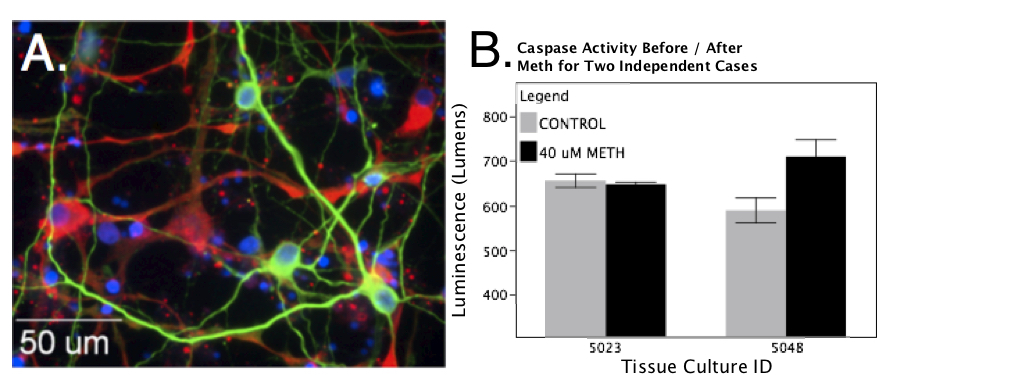
\includegraphics[width=8.2cm]{Figures/Fig1.jpg}
%	\caption{\footnotesize Example wrapped figure. (A) Impressive microscopy image. (B) Impressive data.}
%	\label{fig:example}
%\end{wrapfigure}
%
%Referencing a figure using it's label: Figure \ref{fig:example}. Proin lobortis efficitur dictum. Pellentesque vitae pharetra eros, quis dignissim magna. Sed tellus leo, semper non vestibulum vel, tincidunt eu mi. Aenean pretium ut velit sed facilisis. Ut placerat urna facilisis dolor suscipit vehicula. Ut ut auctor nunc. Nulla non massa eros. Proin rhoncus arcu odio, eu lobortis metus sollicitudin eu. Duis maximus ex dui, id bibendum diam dignissim id. Aliquam quis lorem lorem. Phasellus sagittis aliquet dolor, vulputate cursus dolor convallis vel. Suspendisse eu tellus feugiat, bibendum lectus quis, fermentum nunc. Nunc euismod condimentum magna nec bibendum. Curabitur elementum nibh eu sem cursus, eu aliquam leo rutrum. Sed bibendum augue sit amet pharetra ullamcorper. Aenean congue sit amet tortor vitae feugiat. Vestibulum vestibulum luctus metus venenatis facilisis. Suspendisse iaculis augue at vehicula ornare. Sed vel eros ut velit fermentum porttitor sed sed massa. Fusce venenatis, metus a rutrum sagittis, enim ex maximus velit, id semper nisi velit eu purus.
%
%\begin{description}
%	\item[A.3. Another subheading:]{optional subtitle.}
%\end{description}
%
%In congue risus leo, in gravida enim viverra id. Donec eros mauris, bibendum vel dui at, tempor commodo augue. In vel lobortis lacus. Nam ornare ullamcorper mauris vel molestie. Maecenas vehicula ornare turpis, vitae fringilla orci consectetur vel. Nam pulvinar justo nec neque egestas tristique. Donec ac dolor at libero congue varius sed vitae lectus. Donec et tristique nulla, sit amet scelerisque orci. Maecenas a vestibulum lectus, vitae gravida nulla. Proin eget volutpat orci. Morbi eu aliquet turpis. Vivamus molestie urna quis tempor tristique. Proin hendrerit sem nec tempor sollicitudin.
%
%\begin{figure}[b] % Figure at bottom of the page ([b] argument, could be "t" for top or "h" for here)
%	\centering
%	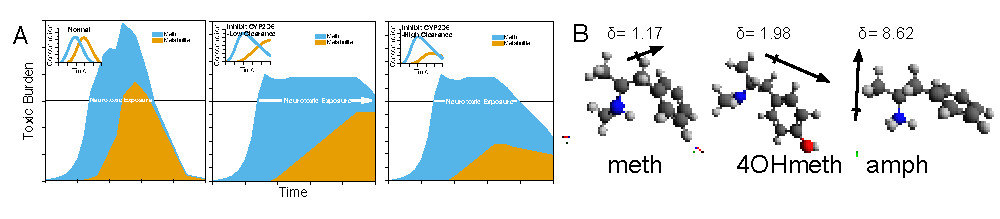
\includegraphics[scale = .80]{Figures/Fig2.pdf}
%	\caption{\footnotesize Big Figure legend Big Figure legend Big Figure legend Big Figure legend Big Figure legend Big Figure legend Big Figure legend Big Figure legend Big Figure legend.}
%	\label{fig2}
%\end{figure}
%
%Fusce eleifend porttitor arcu, id accumsan elit pharetra eget. Mauris luctus velit sit amet est sodales rhoncus. Donec cursus suscipit justo, sed tristique ipsum fermentum nec. Ut tortor ex, ullamcorper varius congue in, efficitur a tellus. Vivamus ut rutrum nisi. Phasellus sit amet enim efficitur, aliquam nulla id, lacinia mauris. Quisque viverra libero ac magna maximus efficitur. Interdum et malesuada fames ac ante ipsum primis in faucibus. Vestibulum mollis eros in tellus fermentum, vitae tristique justo finibus. Sed quis vehicula nibh. Etiam nulla justo, pellentesque id sapien at, semper aliquam arcu. Integer at commodo arcu. Quisque dapibus ut lacus eget vulputate.
%
%Vestibulum sodales orci a nisi interdum tristique. In dictum vehicula dui, eget bibendum purus elementum eu. Pellentesque lobortis mattis mauris, non feugiat dolor vulputate a. Cras porttitor dapibus lacus at pulvinar. Praesent eu nunc et libero porttitor malesuada tempus quis massa. Aenean cursus ipsum a velit ultricies sagittis. Sed non leo ullamcorper, suscipit massa ut, pulvinar erat. Aliquam erat volutpat. Nulla non lacus vitae mi placerat tincidunt et ac diam. Aliquam tincidunt augue sem, ut vestibulum est volutpat eget. Suspendisse potenti. Integer condimentum, risus nec maximus elementum, lacus purus porta arcu, at ultrices diam nisl eget urna. Curabitur sollicitudin diam quis sollicitudin varius. Ut porta erat ornare laoreet euismod. In tincidunt purus dui, nec egestas dui convallis non. In vestibulum ipsum in dictum scelerisque.
%
%\begin{description}
%	\item[A.4. Yet another subheading.]{}
%\end{description}
%
%Aenean feugiat pellentesque venenatis. Sed faucibus tristique tortor vel ultrices. Donec consequat tellus sapien. Nam bibendum urna mauris, eget sagittis justo gravida vel. Mauris nisi lacus, malesuada sit amet neque ut, venenatis tempor orci. Curabitur feugiat sagittis molestie. Duis euismod arcu vitae quam scelerisque facilisis. Praesent volutpat eleifend tortor, in malesuada dui egestas id. Donec finibus ac risus sed pellentesque. Donec malesuada non magna nec feugiat. Mauris eget nibh nec orci congue porttitor vitae eu erat. Sed commodo ipsum ipsum, in elementum neque gravida euismod. Cras mi lacus, pulvinar ut sapien ut, rutrum sagittis dui. Donec non est a metus varius finibus. Pellentesque rutrum pellentesque ligula, vitae accumsan nulla hendrerit ut.
%
%In mi mauris, finibus non faucibus non, imperdiet nec leo. In erat arcu, tincidunt nec aliquam et, volutpat eget nisl. Vivamus id eros scelerisque est condimentum condimentum at at ligula. Proin blandit sapien ac bibendum faucibus. Nunc sem elit, blandit in lectus vitae, lacinia hendrerit risus. Donec efficitur elementum massa, eget interdum nunc porttitor sed. Aenean porttitor gravida nibh, vel bibendum tellus. Nunc fermentum lobortis nunc. Cras aliquet odio mauris, eget lobortis metus lacinia sit amet. Maecenas id elit eu orci ornare ultricies. Sed consequat turpis id accumsan malesuada. Fusce varius imperdiet ex, vel sodales purus scelerisque id. Morbi ut tellus interdum, laoreet leo non, dignissim odio. Nunc vel quam diam. Sed eu tortor in dolor mattis rhoncus.

%----------------------------------------------------------------------------------------
%	INNOVATION
%----------------------------------------------------------------------------------------

%\section*{B. Innovation}
%
%\begin{description}
%	\item[B.1. Instructions.]{}
%\end{description}
%
%Explain how the application challenges and seeks to shift current research or clinical practice paradigms.
%
%Describe any novel theoretical concepts, approaches or methodologies, instrumentation or interventions to be developed or used, and any advantage over existing methodologies, instrumentation, or interventions.
%
%Explain any refinements, improvements, or new applications of theoretical concepts, approaches or methodologies, instrumentation, or interventions.

%----------------------------------------------------------------------------------------
%	APPROACH
%----------------------------------------------------------------------------------------

%\section*{C. Approach}
%
%\begin{description}
%	\item[C.1. Instructions.]{}
%\end{description}
%
%Describe the overall strategy, methodology, and analyses to be used to accomplish the specific aims of the project. Unless addressed separately in Item 15 (Resource Sharing Plan), include how the data will be collected, analyzed, and interpreted as well as any resource sharing plans as appropriate.
%
%Discuss potential problems, alternative strategies, and benchmarks for success anticipated to achieve the aims.
%
%If the project is in the early stages of development, describe any strategy to establish feasibility, and address the management of any high risk aspects of the proposed work.
%
%Point out any procedures, situations, or materials that may be hazardous to personnel and precautions to be exercised. A full discussion on the use of Select Agents should appear in Item 11, below.
%
%As applicable, also include the following information as part of the Research Strategy, keeping within the three sections listed above: Significance, Innovation, and Approach.
%
%\begin{description}
%	\item[C.2. Preliminary Studies for New Applications]{}
%\end{description}
%
%Preliminary Studies for New Applications: For new applications, include information on Preliminary Studies. Discuss the PD/PI's preliminary studies, data, and or experience pertinent to this application. Except for Exploratory/Developmental Grants (R21/R33), Small Research Grants (R03), and Academic Research Enhancement Award (AREA) Grants (R15), preliminary data can be an essential part of a research grant application and help to establish the likelihood of success of the proposed project. Early Stage Investigators should include preliminary data (however, for R01 applications, reviewers will be instructed to place less emphasis on the preliminary data in application from Early Stage Investigators than on the preliminary data in applications from more established investigators).

%----------------------------------------------------------------------------------------
%	PROGRESS REPORT
%----------------------------------------------------------------------------------------

%\newpage
%
%\section*{5. Progress Report Publication List (Renewal Applications Only)}
%
%List the titles and complete references to all appropriate publications, manuscripts accepted for publication, patents, and other printed materials that have resulted from the project since it was last reviewed competitively. When citing articles that fall under the Public Access Policy, were authored or co-authored by the applicant and arose from NIH support, provide the NIH Manuscript Submission reference number (e.g., NIHMS97531) or the Pubmed Central (PMC) reference number (e.g., PMCID234567) for each article. If the PMCID is not yet available because the Journal submits articles directly to PMC on behalf of their authors, indicate "PMC Journal -- In Process." A list of these journals is posted at: http://publicaccess.nih.gov/submit\_process\_journals.htm.
%
%Citations that are not covered by the Public Access Policy, but are publicly available in a free, online format may include URLs or PMCID numbers along with the full reference (note that copies of these publications are not accepted as appendix material, see Part I Section 5.5.15 for more information).

%----------------------------------------------------------------------------------------
%	PROTECTION OF HUMAN SUBJECTS
%----------------------------------------------------------------------------------------

%\newpage
%
%\section*{6. Protection of Human Subjects}
%
%Refer to Part II, Supplemental Instructions for Preparing the Human Subjects Section of the Research Plan.
%
%This section is required for applicants answering "yes" to the question "Are human subjects involved?" on the R\&R Other Project Information form. If the answer is "No" to the question but the proposed research involves human specimens and/or data from subjects applicants must provide a justification in this section for the claim that no human subjects are involved.
%
%Do not use the protection of human subjects section to circumvent the page limits of the Research Strategy.

%----------------------------------------------------------------------------------------
%	INCLUSION OF WOMEN AND MINORITIES
%----------------------------------------------------------------------------------------

%\newpage
%
%\section*{7. Inclusion of Women and Minorities}
%
%Refer to Part II, Supplemental Instructions for Preparing the Human Subjects Section of the Research Plan. This section is required for applicants answering "yes" to the question "Are human subjects involved?" on the R\&R Other Project Information form and the research does not fall under Exemption 4.

%----------------------------------------------------------------------------------------
%	INCLUSION OF CHILDREN
%----------------------------------------------------------------------------------------

%\newpage
%
%%\section*{8. Targeted/Planned Enrollment} - form to fill out 
%\section*{9. Inclusion of Children}
%
%Refer to Supplemental Instructions for Preparing the Human Subjects Section of the Research Plan, Sections 4.4 and 5.7. For applicants answering "Yes" to the question "Are human subjects involved" on the R\&R Other Project Information Form and the research does not fall under Section 4, this section is required.

%----------------------------------------------------------------------------------------
%	VERTEBRATE ANIMALS
%----------------------------------------------------------------------------------------

%\newpage
%
%\section*{10. Vertebrate Animals}
%
%If Vertebrate Animals are involved in the project, address each of the five points below. This section should be a concise, complete description of the animals and proposed procedures. While additional details may be included in the Research Strategy, the responses to the five required points below must be cohesive and include sufficient detail to allow evaluation by peer reviewers and NIH staff. If all or part of the proposed research involving vertebrate animals will take place at alternate sites (such as project/performance or collaborating site(s)), identify those sites and describe the activities at those locations. Although no specific page limitation applies to this section of the application, be succinct. Failure to address the following five points will result in the application being designated as incomplete and will be grounds for the PHS to defer the application from the peer review round. Alternatively, the application’s impact/priority score may be negatively affected.
%
%If the involvement of animals is indefinite, provide an explanation and indicate when it is anticipated that animals will be used. If an award is made, prior to the involvement of animals the grantee must submit to the NIH awarding office detailed information as required in points 1-5 above and verification of IACUC approval. If the grantee does not have an Animal Welfare Assurance then an appropriate Assurance will be required (See Part III, Section 2.2 Vertebrate Animals for more information).
%The five points are as follows:
%
%\begin{enumerate}
%	\item Provide a detailed description of the proposed use of the animals in the work outlined in the Research Strategy section. Identify the species, strains, ages, sex, and numbers of animals to be used in the proposed work.
%	\item Justify the use of animals, the choice of species, and the numbers to be used. If animals are in short supply, costly, or to be used in large numbers, provide an additional rationale for their selection and numbers.
%	\item Provide information on the veterinary care of the animals involved.
%	\item Describe the procedures for ensuring that discomfort, distress, pain, and injury will be limited to that which is unavoidable in the conduct of scientifically sound research. Describe the use of analgesic, anesthetic, and tranquilizing drugs and/or comfortable restraining devices, where appropriate, to minimize discomfort, distress, pain, and injury.
%	\item Describe any method of euthanasia to be used and the reasons for its selection. State whether this method is consistent with the recommendations of the American Veterinary Medical Association (AVMA) Guidelines on Euthanasia. If not, include a scientific justification for not following the recommendations.
%\end{enumerate}
%
%Do not use the vertebrate animal section to circumvent the page limits of the Research Strategy.

%----------------------------------------------------------------------------------------
%	SELECT AGENT RESEARCH
%----------------------------------------------------------------------------------------

%\newpage
%
%\section*{11. Select Agent Research}
%
%Select Agents are hazardous biological agents and toxins that have been identified by DHHS or USDA as having the potential to pose a severe threat to public health and safety, to animal and plant health, or to animal and plant products. CDC maintains a list of these agents. See http://www.cdc.gov/od/sap/docs/salist.pdf.

%----------------------------------------------------------------------------------------
%	MULTIPLE PD/PI LEADERSHIP PLAN
%----------------------------------------------------------------------------------------

%\newpage
%
%\section*{12. Multiple PD/PI Leadership Plan}
%
%For applications designating multiple PD/PIs, a leadership plan must be included. A rationale for choosing a multiple PD/PI approach should be described. The governance and organizational structure of the leadership team and the research project should be described, including communication plans, process for making decisions on scientific direction, and procedures for resolving conflicts. The roles and administrative, technical, and scientific responsibilities for the project or program should be delineated for the PD/PIs and other collaborators.
%
%If budget allocation is planned, the distribution of resources to specific components of the project or the individual PD/PIs should be delineated in the Leadership Plan. In the event of an award, the requested allocations may be reflected in a footnote on the Notice of Grant Award.

%----------------------------------------------------------------------------------------
%	CONSORTIUM/CONTRACTUAL ARRANGEMENTS
%----------------------------------------------------------------------------------------

%\newpage
%
%\section*{13. Consortium/Contractual Arrangements}
%
%Explain the programmatic, fiscal, and administrative arrangements to be made between the applicant organization and the consortium organization(s). If consortium/contractual activities represent a significant portion of the overall project, explain why the applicant organization, rather than the ultimate performer of the activities, should be the grantee. The signature of the Authorized Organization Representative on the SF424 (R\&R) cover component (Item 17) signifies that the applicant and all proposed consortium participants understand and agree to the following statement:
%
%\emph{The appropriate programmatic and administrative personnel of each organization involved in this grant application are aware of the agency's consortium agreement policy and are prepared to establish the necessary inter-organizational agreement(s) consistent with that policy.}

%----------------------------------------------------------------------------------------
%	RESOURCE SHARING
%----------------------------------------------------------------------------------------

%\newpage
%
%%   \section*{14. Letters of Support} - letters to attach
%\section*{15. Resource Sharing}
%
%NIH considers the sharing of unique research resources developed through NIH-sponsored research an important means to enhance the value and further the advancement of the research. When resources have been developed with NIH funds and the associated research findings published or provided to NIH, it is important that they be made readily available for research purposes to qualified individuals within the scientific community. See Part III, 1.5 Sharing Research Resources.
%
%\begin{enumerate}
%	\item{Data Sharing Plan:} Investigators seeking \$500,000 or more in direct costs (exclusive of consortium F\&A) in any year are expected to include a brief 1-paragraph description of how final research data will be shared, or explain why data-sharing is not possible. Specific Funding Opportunity Announcements may require that all applications include this information regardless of the dollar level. Applicants are encouraged to read the specific opportunity carefully and discuss their data-sharing plan with their program contact at the time they negotiate an agreement with the Institute/Center (IC) staff to accept assignment of their application. See Data-Sharing Policy or http://grants.nih.gov/grants/guide/notice- files/NOT-OD-03-032.html.
%	\item{Sharing Model Organisms:} Regardless of the amount requested, all applications where the development of model organisms is anticipated are expected to include a description of a specific plan for sharing and distributing unique model organisms or state why such sharing is restricted or not possible. See Sharing Model Organisms Policy, and NIH Guide NOT-OD-04-042.
%	\item{Genome Wide Association Studies (GWAS):} Applicants seeking funding for a genome-wide association study are expected to provide a plan for submission of GWAS data to the NIH-designated GWAS data repository, or an appropriate explanation why submission to the repository is not possible. GWAS is defined as any study of genetic variation across the entire genome that is designed to identify genetic associations with observable traits (such as blood pressure or weight) or the presence or absence of a disease or condition. For further information see Policy for Sharing of Data Obtained in NIH Supported or Conducted Genome-Wide Association Studies, NIH Guide NOT-OD-07-088, and http://grants.nih.gov/grants/gwas/.
%\end{enumerate}
